\documentclass[12pt]{article}
\usepackage{graphicx}
\usepackage{amssymb}
\usepackage{epstopdf}
\usepackage{amsmath}
\usepackage{multicol}
\usepackage{tcolorbox}
\usepackage{geometry}
\usepackage{enumitem}
\usepackage{fancyhdr}

\DeclareGraphicsRule{.tif}{png}{.png}{`convert #1 `dirname #1`/`basename #1 .tif`.png}

\textwidth = 6.5 in
\textheight = 9 in
\oddsidemargin = 0.0 in
\evensidemargin = 0.0 in
\topmargin = -23pt
\headheight = 0.0 in
\headsep = 0.0 in
\parskip = 0.2in
\parindent = 0.0in
\pagestyle{fancy}
\pagenumbering{gobble}

\newtheorem{theorem}{Theorem}
\newtheorem{corollary}[theorem]{Corollary}
\newtheorem{definition}{Definition}
%\includegraphics [height=50mm, width=50mm]{PathInt.jpg}
\title{Title} 

\begin{document}
%INSTRUCTOR NOTES

 Name:
 \begin{center}\large{3.5 Derivatives of Trigonometric Functions}\end{center}
 

 \begin{tcolorbox}
 
\bf{Warm-up:} Compute the following derivatives:
 	\begin{enumerate}
	\item $\displaystyle \frac{d}{dt}\left(\frac{x^{2}}{2^{3x}}\right)$
\vfill
	\item $\displaystyle \frac{d}{dx}\left(\sin\left(xe^{x}\right)\right)$
	\vfill
	
	\end{enumerate}
 \end{tcolorbox}
	
 \begin{enumerate}
\item Sketch a derivative function for each of the functions shown below. What do you notice?

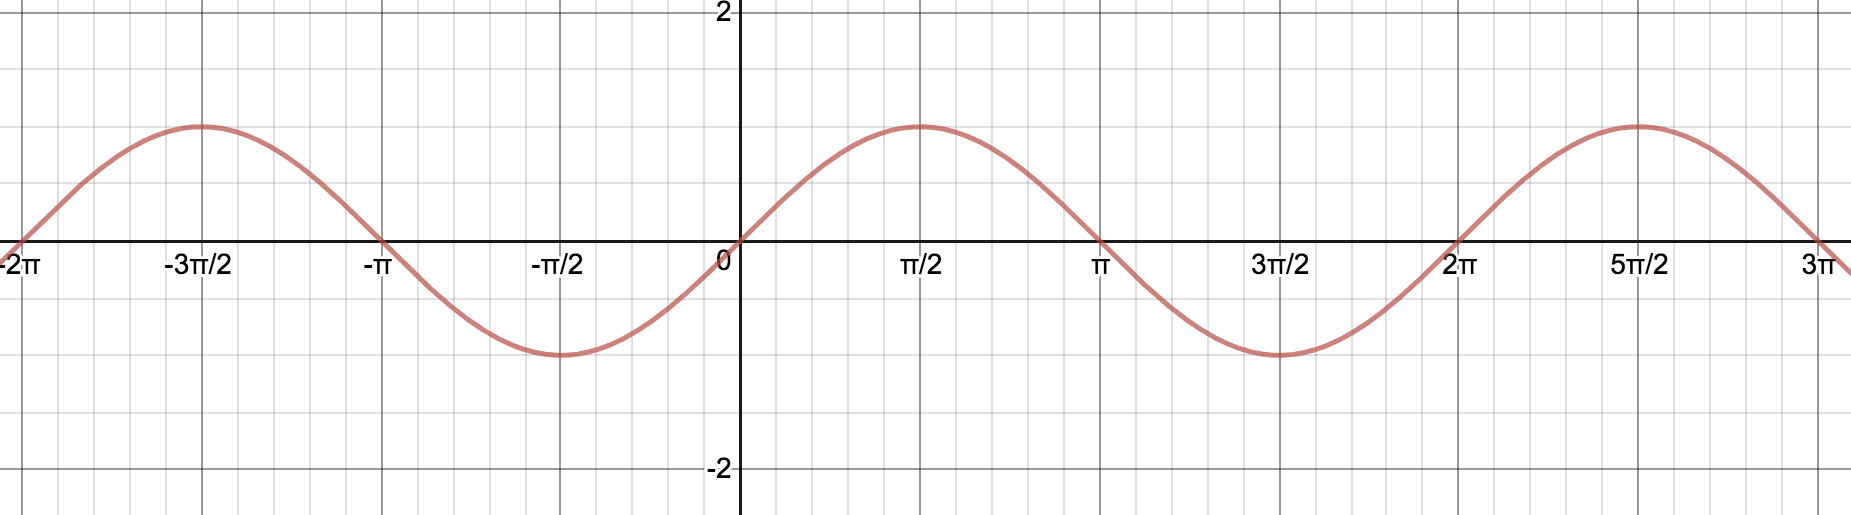
\includegraphics [height=30mm, width=120mm]{3_5_sin}\\

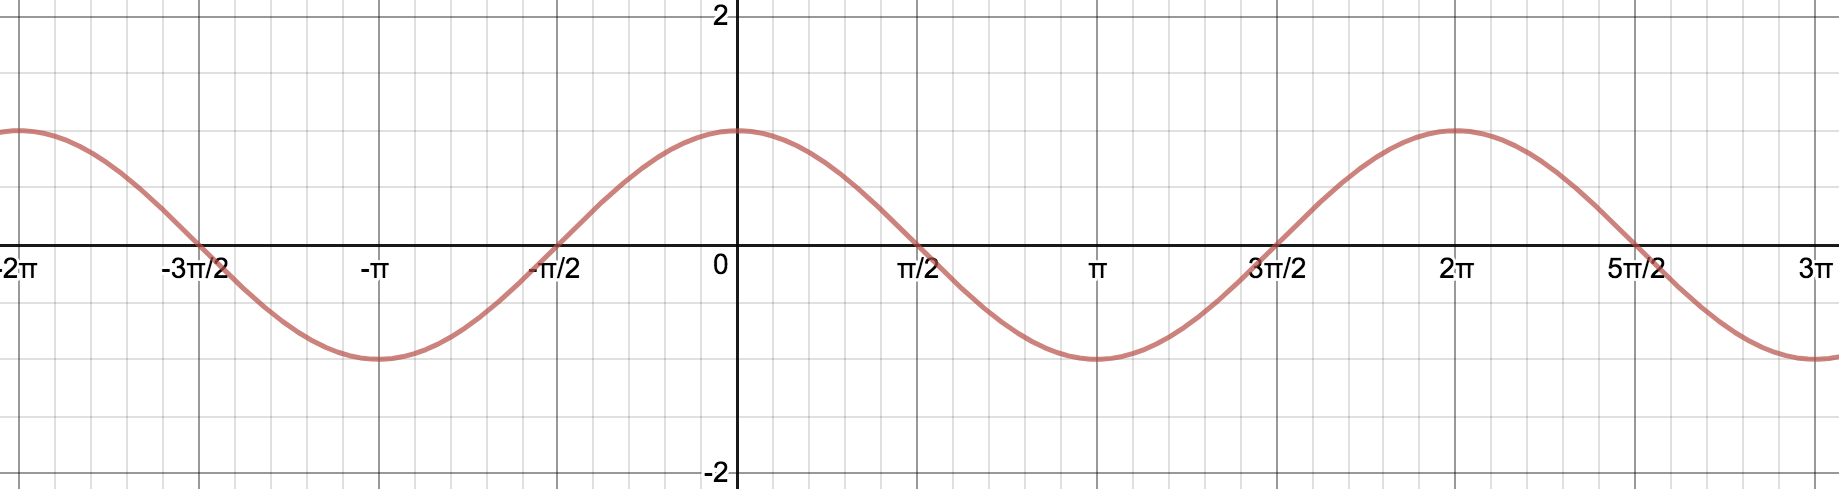
\includegraphics [height=30mm, width=120mm]{3_5_cos}\\
\vfill

\begin{tcolorbox}

\textbf{Derivatives of Trigonometric Functions} \\
\begin{multicols}{2}
\begin{enumerate}[itemsep=1cm]
\item $\displaystyle \frac{d}{d\theta} \sin(\theta) = $
\item $\displaystyle \frac{d}{d\theta} \cos(\theta) = $
\item $\displaystyle \frac{d}{d\theta} \tan(\theta) = $\\
\item $\displaystyle \frac{d}{d\theta} \csc(\theta) = $
\item $\displaystyle \frac{d}{d\theta} \sec(\theta) = $
\item $\displaystyle \frac{d}{d\theta} \cot(\theta) = $\\
\end{enumerate}
\end{multicols}

\end{tcolorbox}

\newpage

$\hspace{10px}$ \\

\item  Compute the following derivatives. 
\begin{enumerate}
	\item $\displaystyle \frac{d}{d\theta}\left[\theta\tan\theta\right]$
	\vfill
	\item $\displaystyle \frac{d}{dx}\left[\cos^{2}\left(x\right)\right]$
	\vfill
	\item $\displaystyle \frac{d}{dt}\left[\sin\left(3^{t}\right)\cos\left(2^{t}\right)\right]$
	\vfill
	\end{enumerate}

\vfill
\item The depth, $y$, in feet, of water in Newport Harbor is given in terms of $t$, the number of hours since midnight, by

$$y=5+4.9\cos\left(\frac{\pi}{6}t\right).$$
	\begin{enumerate}
	\item  Find $\displaystyle \frac{dy}{dt}$. What does $\displaystyle \frac{dy}{dt}$ represent, in terms of water level?
	
	\vfill
	\item For $0\le t\le24$, when is $\displaystyle \frac{dy}{dt}$ zero?  Explain what it means (in terms of water level) for $\displaystyle \frac{dy}{dt}$ to be zero.
	\end{enumerate}

\end{enumerate}
\end{document} 
A company charges a flat rate of \$500 to rent up to 100 chairs and every additional chair costs \$4. Draw a graph and find a formula for the cost $C$ as a function of $n$, the number of chairs rented.\\
%%%%%%%%%
\begin{tcolorbox}
\textbf{Warm-up: } Solve the following equations for $t$.
\begin{multicols}{2}
\begin{enumerate}
\item $(t+1)^2=9$
\item $tx+x^2=5$
\end{enumerate}
\end{multicols}
\end{tcolorbox}	

MINIPAGE
\noindent\begin{minipage}{0.3\textwidth}% adapt widths of minipages to your needs
try 1
\end{minipage}%
\hspace{40mm}
\begin{minipage}{0.6\textwidth}
a) $f'(2)=$\\\

b) $f'(4)=$\\

c) $f'(6)=$\\

d) $f'(7)=$\\

e) $f'(8)=$
\end{minipage}
